\documentclass[aspectratio=169]{beamer}

% ---------- fonts & basics ----------
\usepackage[T1]{fontenc}
\usepackage{helvet}
\renewcommand{\familydefault}{\sfdefault}
\usepackage{graphicx}
\usepackage{amsmath,amssymb}

% ---------- tikz ----------
\usepackage{tikz}
\usetikzlibrary{arrows.meta, positioning, calc, shapes.geometric,
                backgrounds, fit, decorations.pathreplacing, shadows}

% ---------- beamer look ----------
\setbeamertemplate{navigation symbols}{}
\setbeamertemplate{footline}{}
\definecolor{navy}{HTML}{1B2A4A}
\definecolor{slategray}{HTML}{5B6B84}
\setbeamercolor{frametitle}{fg=navy,bg=white}
\setbeamerfont{frametitle}{series=\bfseries,size=\large}
\setbeamercolor{normal text}{fg=navy}

% ---------- palette ----------
\definecolor{amber}{HTML}{C8850C}
\definecolor{amberlight}{HTML}{FBF0DA}
\definecolor{skyblue}{HTML}{2E75B6}
\definecolor{skybluelight}{HTML}{E9F2FA}
\definecolor{coral}{HTML}{D4552A}
\definecolor{corallight}{HTML}{FBE9E1}
\definecolor{violet}{HTML}{6449B6}
\definecolor{violetlight}{HTML}{F0ECFA}
\definecolor{ghostgray}{HTML}{C9CFD8}
\definecolor{tealmem}{HTML}{1E7F72}
\definecolor{tealmemlight}{HTML}{E4F3F0}

% ---------- reusable tikz styles ----------
\tikzset{
  >={Latex[length=2.1mm,width=1.5mm]},
  flow/.style={-{Latex[length=2.1mm,width=1.5mm]}, thick, draw=slategray},
  dashedflow/.style={-{Latex[length=1.8mm,width=1.3mm]}, thick, dashed, draw=slategray!70},
  imgcard/.style={draw=slategray!60, thick, rounded corners=1.5pt, fill=white,
                  minimum width=1.15cm, minimum height=1.15cm, inner sep=0pt},
  procbox/.style={rounded corners=3pt, draw=coral, line width=0.9pt, fill=corallight,
                   align=center, text=navy, font=\scriptsize, text width=2.4cm,
                   minimum height=1.4cm, inner sep=4pt},
  eqbox/.style={rounded corners=3pt, draw=violet, line width=0.9pt, fill=violetlight,
                   align=center, text=navy, font=\scriptsize, text width=6.4cm,
                   minimum height=1.5cm, inner sep=5pt},
  notebox/.style={rounded corners=3pt, draw=amber!55, line width=0.7pt, fill=amberlight!55,
                   align=center, text=navy, font=\scriptsize, inner sep=5pt},
  smallcaption/.style={font=\tiny, text=slategray, align=center},
  % large matrix cell (identical to the deck's Figure 2)
  numcell/.style={draw=slategray!45, thin, minimum width=6.6mm, minimum height=6.2mm,
                   inner sep=0pt, font=\fontsize{5}{5}\selectfont, text=navy},
  % compact numbered cell (for the scoring figure)
  numcellS/.style={draw=slategray!45, thin, minimum width=6.0mm, minimum height=5.4mm,
                   inner sep=0pt, font=\fontsize{4.6}{4.6}\selectfont, text=navy},
  cropcard/.style={draw=slategray!60, thick, rounded corners=1.5pt, fill=white,
                   minimum width=0.95cm, minimum height=0.95cm, inner sep=0pt},
  candbox/.style={draw=coral, line width=1.0pt},
  gtbox/.style={draw=tealmem, line width=1.2pt},
  imgph/.style={draw=slategray!60, line width=0.55pt, rounded corners=1.5pt, fill=white,
                   inner sep=0pt, minimum width=0.62cm, minimum height=0.62cm},
}

% ---- compact numbered rows (same look as the deck's Figs 5, 6) ----
\newcommand{\cwS}{0.62}
\newcommand{\shrowN}[3]{%
  \foreach \v [count=\ic from 0] in {#2}{%
    \ifnum\ic<4\relax
      \node[numcellS, fill=#1] at (\ic*\cwS,0){\v};%
    \else
      \pgfmathsetmacro{\xx}{4*\cwS+0.34+(\ic-4)*\cwS}%
      \node[numcellS, fill=#1] at (\xx,0){\v};%
    \fi
  }%
  \node[font=\tiny, text=slategray] at (4*\cwS-0.14,0){$\cdots$};%
  \node[font=\scriptsize, text=navy, anchor=west] at (5.15,0){#3};%
}
\newcommand{\sbracketsC}[3]{%
  \draw[line width=0.8pt, draw=#1] (-0.36,#2) ++(0.18,0) -- (-0.36,#2) -- (-0.36,#3) -- ++(0.18,0);%
  \draw[line width=0.8pt, draw=#1] (5.02,#2) ++(-0.18,0) -- (5.02,#2) -- (5.02,#3) -- ++(-0.18,0);%
}

\begin{document}

% =====================================================
% FIGURE 2b : DISTRACTOR-BANK CONSTRUCTION  (sibling of Figure 2)
% =====================================================
\begin{frame}{Figure 2b --- Distractor Bank: Red Detections $\to$ OSNet $\to$ Negative Matrix}

\centering
\resizebox{!}{0.86\textheight}{%
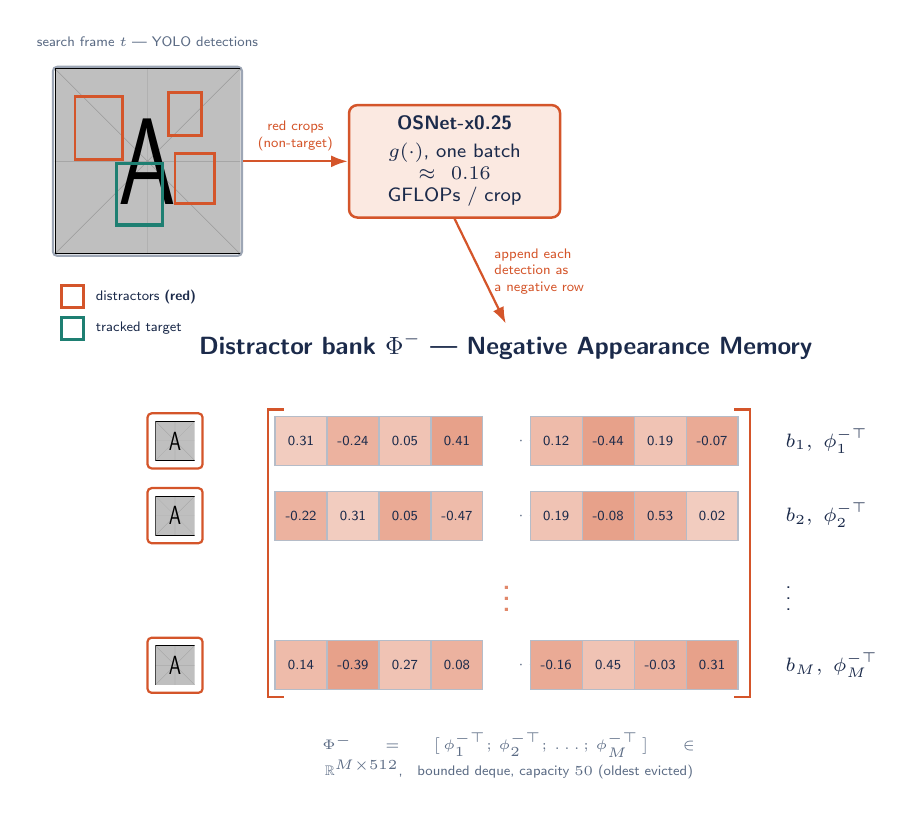
\begin{tikzpicture}[font=\small, x=1cm, y=1cm]

\def\rowspacing{0.95}
\def\cw{0.66}

% =========== STAGE 1 : annotated frame -> OSNet ===========
\node[imgcard, minimum width=2.4cm, minimum height=2.4cm] (frame) at (0,0)
      {\includegraphics[width=2.35cm,height=2.35cm]{example-image-a}};
\node[smallcaption, above=1.2mm of frame] {search frame $t$ --- YOLO detections};
% distractor detections (red)
\node[candbox, minimum width=0.60cm, minimum height=0.80cm] at (-0.62,0.42) {};
\node[candbox, minimum width=0.50cm, minimum height=0.64cm] at (0.60,-0.22) {};
\node[candbox, minimum width=0.42cm, minimum height=0.54cm] at (0.48,0.60) {};
% tracked target (teal)
\node[gtbox, minimum width=0.58cm, minimum height=0.78cm] at (-0.10,-0.42) {};
% legend
\node[candbox, minimum width=0.28cm, minimum height=0.28cm] at (-0.95,-1.72) {};
\node[font=\tiny, text=navy, anchor=west] at (-0.78,-1.72) {distractors \textbf{(red)}};
\node[gtbox, minimum width=0.28cm, minimum height=0.28cm] at (-0.95,-2.12) {};
\node[font=\tiny, text=navy, anchor=west] at (-0.78,-2.12) {tracked target};

\node[procbox] (osnet) at (3.9,0) {\textbf{OSNet-x0.25}\\[2pt]{\scriptsize $g(\cdot)$, one batch}\\{\scriptsize $\approx0.16$ GFLOPs / crop}};
\draw[flow, draw=coral] (frame.east) --
      node[above, font=\tiny, text=coral, align=center]{red crops\\ (non-target)} (osnet.west);

% =========== STAGE 2 : route into the bank ===========
\coordinate (matOrigin) at (1.95,-3.55);
\node[navy, font=\bfseries\small] (banktitle) at (4.55,-2.35)
      {Distractor bank $\Phi^{-}$ --- Negative Appearance Memory};
\draw[flow, draw=coral] (osnet.south) -- node[right, font=\tiny, text=coral, xshift=0.5mm, align=left]
      {append each\\ detection as\\ a negative row} (banktitle.north);

% =========== STAGE 3 : the stacked negative matrix ===========
% -- row 1 --
\begin{scope}[shift={(matOrigin)}]
  \node[imgcard, draw=coral, minimum width=7mm, minimum height=7mm] at (-1.6,0)
        {\includegraphics[width=5mm,height=5mm]{example-image-a}};
  \foreach \i/\v/\c in {0/{0.31}/coral!30,1/{-0.24}/coral!45,2/{0.05}/coral!35,3/{0.41}/coral!55}{
    \node[numcell, fill=\c] at (\i*\cw,0) {\v};}
  \node[font=\tiny, text=slategray] at (4*\cw+0.3,0) {$\cdots$};
  \foreach \i/\v/\c in {0/{0.12}/coral!40,1/{-0.44}/coral!55,2/{0.19}/coral!35,3/{-0.07}/coral!50}{
    \node[numcell, fill=\c] at (4*\cw+0.6+\i*\cw,0) {\v};}
  \node[font=\scriptsize, text=navy, anchor=west] at (8*\cw+0.75,0) {$b_1,\ \phi_1^{-\top}$};
\end{scope}
% -- row 2 --
\begin{scope}[shift={($(matOrigin)+(0,-\rowspacing)$)}]
  \node[imgcard, draw=coral, minimum width=7mm, minimum height=7mm] at (-1.6,0)
        {\includegraphics[width=5mm,height=5mm]{example-image-a}};
  \foreach \i/\v/\c in {0/{-0.22}/coral!45,1/{0.31}/coral!30,2/{0.05}/coral!50,3/{-0.47}/coral!40}{
    \node[numcell, fill=\c] at (\i*\cw,0) {\v};}
  \node[font=\tiny, text=slategray] at (4*\cw+0.3,0) {$\cdots$};
  \foreach \i/\v/\c in {0/{0.19}/coral!35,1/{-0.08}/coral!55,2/{0.53}/coral!45,3/{0.02}/coral!30}{
    \node[numcell, fill=\c] at (4*\cw+0.6+\i*\cw,0) {\v};}
  \node[font=\scriptsize, text=navy, anchor=west] at (8*\cw+0.75,0) {$b_2,\ \phi_2^{-\top}$};
\end{scope}
% -- ellipsis row --
\node[font=\Large, text=coral!70] at ($(matOrigin)+(3.5*\cw+0.3,-2*\rowspacing)$) {$\vdots$};
\node[font=\scriptsize, text=navy, anchor=west] at ($(matOrigin)+(8*\cw+0.75,-2*\rowspacing)$) {$\vdots$};
% -- row M --
\begin{scope}[shift={($(matOrigin)+(0,-3*\rowspacing)$)}]
  \node[imgcard, draw=coral, minimum width=7mm, minimum height=7mm] at (-1.6,0)
        {\includegraphics[width=5mm,height=5mm]{example-image-a}};
  \foreach \i/\v/\c in {0/{0.14}/coral!40,1/{-0.39}/coral!55,2/{0.27}/coral!35,3/{0.08}/coral!45}{
    \node[numcell, fill=\c] at (\i*\cw,0) {\v};}
  \node[font=\tiny, text=slategray] at (4*\cw+0.3,0) {$\cdots$};
  \foreach \i/\v/\c in {0/{-0.16}/coral!50,1/{0.45}/coral!35,2/{-0.03}/coral!45,3/{0.31}/coral!55}{
    \node[numcell, fill=\c] at (4*\cw+0.6+\i*\cw,0) {\v};}
  \node[font=\scriptsize, text=navy, anchor=west] at (8*\cw+0.75,0) {$b_M,\ \phi_M^{-\top}$};
\end{scope}

% ---- big matrix brackets spanning all rows ----
\coordinate (bTL) at ($(matOrigin)+(-0.42, 0.40)$);
\coordinate (bBL) at ($(matOrigin)+(-0.42,-3*\rowspacing-0.40)$);
\coordinate (bTR) at ($(matOrigin)+(8*\cw+0.42, 0.40)$);
\coordinate (bBR) at ($(matOrigin)+(8*\cw+0.42,-3*\rowspacing-0.40)$);
\draw[line width=0.9pt, draw=coral] ($(bTL)+(0.2,0)$) -- (bTL) -- (bBL) -- ++(0.2,0);
\draw[line width=0.9pt, draw=coral] ($(bTR)+(-0.2,0)$) -- (bTR) -- (bBR) -- ++(-0.2,0);

\node[smallcaption, text width=8.4cm] at ($(matOrigin)+(2.64,-3*\rowspacing-1.15)$)
      {$\Phi^{-}=\big[\,\phi_1^{-\top};\,\phi_2^{-\top};\,\ldots;\,\phi_M^{-\top}\,\big]\in\mathbb{R}^{M\times512}$,\quad
       bounded deque, capacity $50$ (oldest evicted)};

\end{tikzpicture}%
}

\end{frame}

% =====================================================
% FIGURE 8 : DISTRACTOR-AWARE DRM SCORING (the subtraction hint)
% =====================================================
\begin{frame}{Figure 8 --- Distractor-Aware Scoring: Subtract the Distractor Match}

\centering
\vspace{1mm}
\resizebox{0.99\textwidth}{!}{%
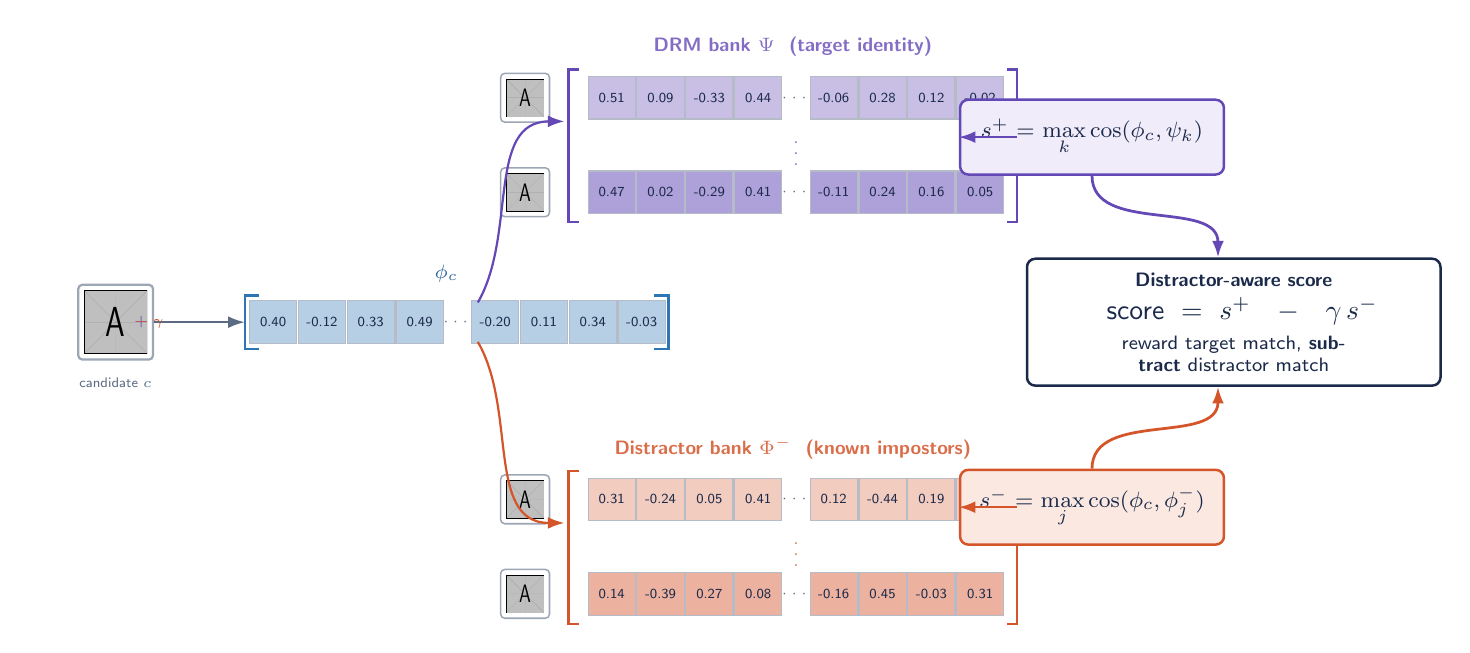
\begin{tikzpicture}[font=\small, x=1cm, y=1cm]

% ---- candidate embedding (center-left) ----
\node[cropcard] (cc) at (0,0) {\includegraphics[width=0.8cm,height=0.8cm]{example-image-a}};
\node[smallcaption, below=1mm of cc, text width=2.0cm]{candidate $c$};
\begin{scope}[shift={(2.0,0)}]
  \shrowN{skyblue!35}{0.40,-0.12,0.33,0.49,-0.20,0.11,0.34,-0.03}{}
  \sbracketsC{skyblue}{0.34}{-0.34}
\end{scope}
\node[font=\scriptsize, text=skyblue!85!black] at (4.2,0.62) {$\phi_c$};
\draw[flow] (cc.east) -- (1.64,0);

% ================= TOP branch : DRM target bank (reward) =================
\begin{scope}[shift={(6.3,2.55)}]
  \node[violet!80, font=\bfseries\scriptsize] at (2.3,0.95) {DRM bank $\Psi$ \ (target identity)};
  \begin{scope}[shift={(0,0.30)}]
    \node[imgph] at (-1.1,0){\includegraphics[width=0.48cm,height=0.48cm]{example-image-a}};
    \shrowN{violet!35}{0.51,0.09,-0.33,0.44,-0.06,0.28,0.12,-0.02}{}
  \end{scope}
  \node[font=\scriptsize, text=violet!70] at (4*\cwS-0.14,-0.30){$\vdots$};
  \begin{scope}[shift={(0,-0.90)}]
    \node[imgph] at (-1.1,0){\includegraphics[width=0.48cm,height=0.48cm]{example-image-a}};
    \shrowN{violet!52}{0.47,0.02,-0.29,0.41,-0.11,0.24,0.16,0.05}{}
  \end{scope}
  \draw[line width=0.8pt, draw=violet] (-0.42,0.66) -- (-0.55,0.66) -- (-0.55,-1.28) -- (-0.42,-1.28);
  \draw[line width=0.8pt, draw=violet] (5.02,0.66) -- (5.15,0.66) -- (5.15,-1.28) -- (5.02,-1.28);
\end{scope}
\node[eqbox, draw=violet, fill=violetlight, text width=3.0cm, minimum height=0.95cm] (splus)
      at (12.4,2.35)
      {\footnotesize$s^{+}=\displaystyle\max_{k}\cos(\phi_c,\psi_k)$};
\draw[flow, draw=violet] (4.6,0.25) to[out=60,in=180] (6.3-0.6,2.55);
\draw[flow, draw=violet] (6.3+5.15,2.35) -- (splus.west);

% ================= BOTTOM branch : distractor bank (penalty) =================
\begin{scope}[shift={(6.3,-2.55)}]
  \node[coral!85, font=\bfseries\scriptsize] at (2.3,0.95) {Distractor bank $\Phi^{-}$ \ (known impostors)};
  \begin{scope}[shift={(0,0.30)}]
    \node[imgph] at (-1.1,0){\includegraphics[width=0.48cm,height=0.48cm]{example-image-a}};
    \shrowN{coral!30}{0.31,-0.24,0.05,0.41,0.12,-0.44,0.19,-0.07}{}
  \end{scope}
  \node[font=\scriptsize, text=coral!70] at (4*\cwS-0.14,-0.30){$\vdots$};
  \begin{scope}[shift={(0,-0.90)}]
    \node[imgph] at (-1.1,0){\includegraphics[width=0.48cm,height=0.48cm]{example-image-a}};
    \shrowN{coral!45}{0.14,-0.39,0.27,0.08,-0.16,0.45,-0.03,0.31}{}
  \end{scope}
  \draw[line width=0.8pt, draw=coral] (-0.42,0.66) -- (-0.55,0.66) -- (-0.55,-1.28) -- (-0.42,-1.28);
  \draw[line width=0.8pt, draw=coral] (5.02,0.66) -- (5.15,0.66) -- (5.15,-1.28) -- (5.02,-1.28);
\end{scope}
\node[eqbox, draw=coral, fill=corallight, text width=3.0cm, minimum height=0.95cm] (sminus)
      at (12.4,-2.35)
      {\footnotesize$s^{-}=\displaystyle\max_{j}\cos(\phi_c,\phi^{-}_{j})$};
\draw[flow, draw=coral] (4.6,-0.25) to[out=-60,in=180] (6.3-0.6,-2.55);
\draw[flow, draw=coral] (6.3+5.15,-2.35) -- (sminus.west);

% ================= COMBINE : score = s+ - gamma s- =================
\node[eqbox, text width=4.9cm, minimum height=1.55cm, draw=navy, fill=white] (score) at (14.2,0)
      {\textbf{Distractor-aware score}\\[4pt]
       {\normalsize$\;\text{score}=s^{+}\;-\;\gamma\, s^{-}$}\\[3pt]
       {\scriptsize reward target match, \textbf{subtract} distractor match}};
\draw[flow, draw=violet, line width=1pt] (splus.south) to[out=-90,in=90] ($(score.north)+(-0.2,0)$)
      node[midway, right=1mm, font=\tiny, text=violet]{$+$};
\draw[flow, draw=coral, line width=1pt] (sminus.north) to[out=90,in=-90] ($(score.south)+(-0.2,0)$)
      node[midway, right=1mm, font=\tiny, text=coral]{$-\,\gamma$};

\end{tikzpicture}%
}

\vspace{2mm}
\begin{center}\begin{minipage}{0.92\textwidth}\centering

\begin{tikzpicture}\node[notebox, text width=0.97\textwidth]{%
A look-alike in the right place still scores high on the target bank $s^{+}$ --- but if it also matches a
\textbf{banked distractor} it earns a large $s^{-}$, and $-\gamma s^{-}$ \textbf{pulls its score back down}.
Only a candidate that matches the target \emph{and} none of the known impostors survives.};\end{tikzpicture}
\end{minipage}\end{center}

\end{frame}

\end{document}
